\documentclass[dvipsnames]{article}
\usepackage{tikz,pgfplots}
\usepackage{tikz-qtree}
\usepackage{units}
\usepackage{braket}
\usepackage[]{xcolor}
\pgfplotsset{compat=1.8}
%\pgfplotsset{colormap={mix}{
%	color(0cm)=(blue);
%	color(1cm)=(green);
%	color(2cm)=(yellow)
%	color(3cm)=(red)}}

\usetikzlibrary{patterns,shadows,fadings,positioning,trees,calc}
\usepgfplotslibrary{external}
\tikzexternalize


\tikzfading[name=fade inside,
         inner color=transparent!80,
         outer color=transparent!30]
\tikzfading[name=fade out,
         inner color=transparent!0,
         outer color=transparent!90]


%\definecolor{diplom1}{rgb}{0.0 0.4 1.0}
%\definecolor{diplom2}{rgb}{0.0 0.0 0.6}
\definecolor{diplom1}{RGB}{101 156 239}
\definecolor{diplom2}{RGB}{000 000 128}
\definecolor{diplom3}{RGB}{153,0,0} %unirot
\definecolor{diplom4}{RGB}{232,215,23}
\definecolor{diplom5}{RGB}{51,37,60}

\definecolor{unirot}{RGB}{153,0,0}
\definecolor{unirot_hell}{RGB}{255,228,225}
\definecolor{lightblue}{RGB}{242.2,249.88,255}

\pgfplotsset{colormap={diplom1s}{
       color(0cm)=(white);
       color(1cm)=(diplom1);
       color(10cm)=(diplom1)}}
\pgfplotsset{colormap={diplom2s}{
       color(0cm)=(white);
       color(1cm)=(diplom1);
       color(2cm)=(diplom2)}}
\pgfplotsset{colormap={blues}{
       color(0cm)=(diplom2);
       color(1cm)=(diplom1);
       color(2cm)=(white);
       color(3cm)=(diplom1);
       color(4cm)=(diplom2)}}

\pgfplotsset{
   /pgfplots/bar  cycle  list/.style={/pgfplots/cycle  list={%
        {diplom1,  fill=diplom1!30!white,  mark=none,very thick},%
        {diplom2,  fill=diplom2!30!white,  mark=none,very thick},%
        {diplom3,  fill=diplom3!30!white,  mark=none,very thick},%
        {orange,   fill=orange!30!white,   mark=none,very thick},%
        {LimeGreen,fill=LimeGreen!30!white,mark=none,very thick},%
        {Fuchsia,  fill=Fuchsia!30!white,  mark=none,very thick},%
        {Green,    fill=Green!30!white,    mark=none,very thick},%
        {Goldenrod,fill=Goldenrod!30!white,mark=none,very thick},%
     }
   },
}

\pgfplotsset{
  cycle  list={%
        {diplom1,  mark=none,very thick},%
        {diplom2,  mark=none,very thick},%
        {diplom3,  mark=none,very thick},%
        {orange,   mark=none,very thick},%
        {LimeGreen,mark=none,very thick},%
        {Fuchsia,  mark=none,very thick},%
        {Green,    mark=none,very thick},%
        {Goldenrod,mark=none,very thick},%
     }
   }


\begin{document}

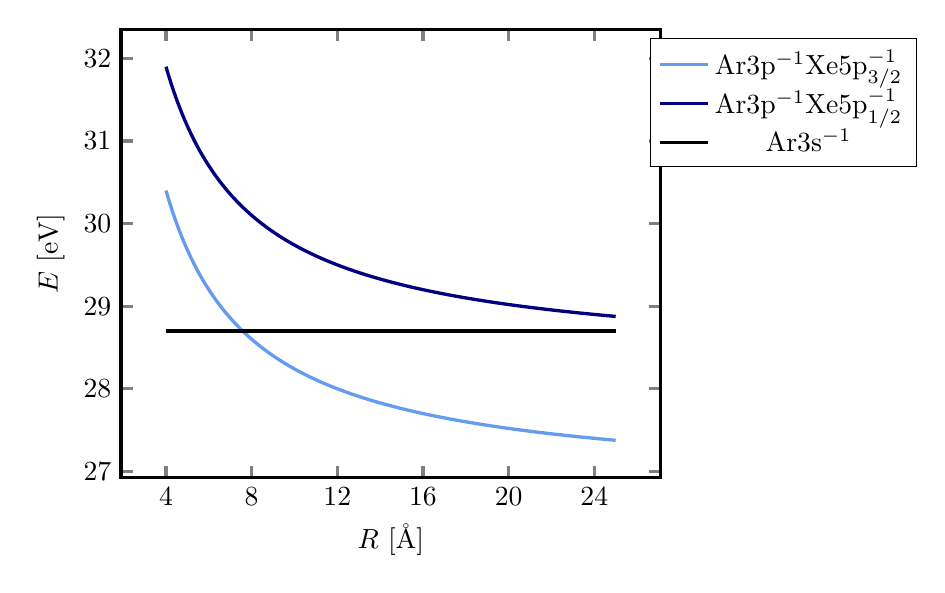
\begin{tikzpicture}
    \begin{axis}[domain=4.0:25,
                 samples = 200,
                 xtick={4.0,8.0,...,24},
                 %xticklabels={$-\pi$,$-\frac \pi 2$,0,$\frac \pi 2$,$\pi$},
                 %cycle list name = exotic,
                 legend style={anchor= north west},
                 xlabel={$R$ [\AA]},
                 ylabel={$E$ [eV]},
                 axis line style = very thick,
                 tick style = very thick,
                 ]

      \addplot+[
                mark = none,
               ]
               {15.3 + 11.5 + 14.39964 / x};
      \addlegendentry{Ar3p$^{-1}$Xe5p$_{3/2}^{-1}$};

      \addplot+[
                mark = none,
               ]
               {15.3 + 13.0 + 14.39964 / x};
      \addlegendentry{Ar3p$^{-1}$Xe5p$_{1/2}^{-1}$};


      \addplot+[
                mark = none,
                black,
               ]
               {28.7};
      \addlegendentry{Ar3s$^{-1}$};
      %\draw[] (axis cs:\pgfkeysvalueof{/pgfplots/xmin},29.239) -- (axis cs:\pgfkeysvalueof{/pgfplots/xmax},29.239);
    \end{axis}
\end{tikzpicture}


\end{document}
